% = = = = = = = = = = = = = = = = = = = = = %
%            Concept Selection              %
% = = = = = = = = = = = = = = = = = = = = = %

\let\clearpage\relax
\chapter{Concept Selection}

\section{ISA}\label{section:isa} %sj
The exist several popular instruction set architectures (ISA), such as x86, MIPS, ARMv7 and RISC-V. As we mentioned before, they can be classified by their architectural complexity. Since complex instruction set computer (CISC) is too complicated, we choose among reduced instruction set computers (RISC). Following are three widely-used reduced instruction set computers.

\begin{enumerate}
\item \textbf{MIPS:} Microprocessor without Interlocked Pipeline Stages (MIPS) is a RISC ISA developed by MIPS Computer System. It is widely used in computer architecture courses for university students. Most of group members are familiar with MIPS Instructions and have develop experience on it.

\begin{figure}[!htp]
    \centering
    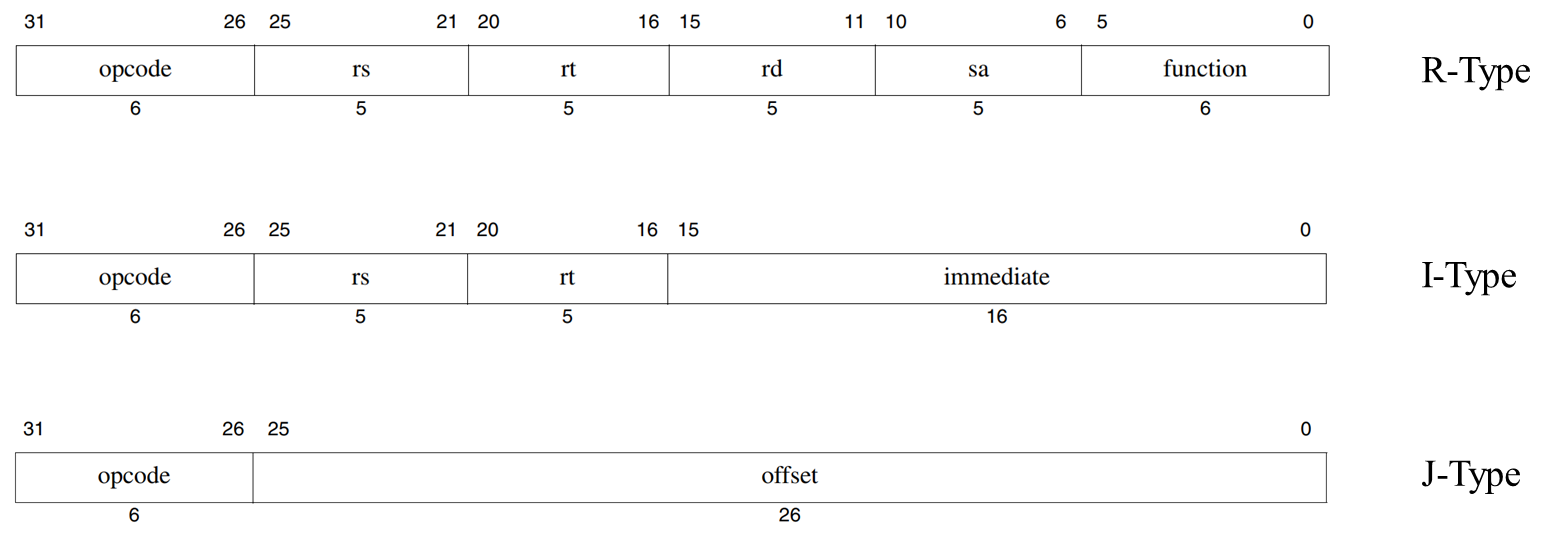
\includegraphics[width=0.7\textwidth]{figure/MIPS-instruction-format-18.png}
    \caption{MIPS instruction format\cite{mips_ist}.}
    \label{fig:mips_inst}
\end{figure}

However, with years of development, the design space of MIPS has been exploited, which will be an obstacle to further research.
\item \textbf{ARMv7:} Advanced RISC Machines (ARM) is a family of RISC ISA developed by Arm Ltd. Among them, ARMv7 is a classic structure that be applied in many areas. Due to its low cost, minimal power consumption, and low heat generation rate, ARMv7 is desirable for light, portable, battery-powered devices, such as smartphoes, laptops and other embedded systems.

\begin{figure}[!htp]
    \centering
    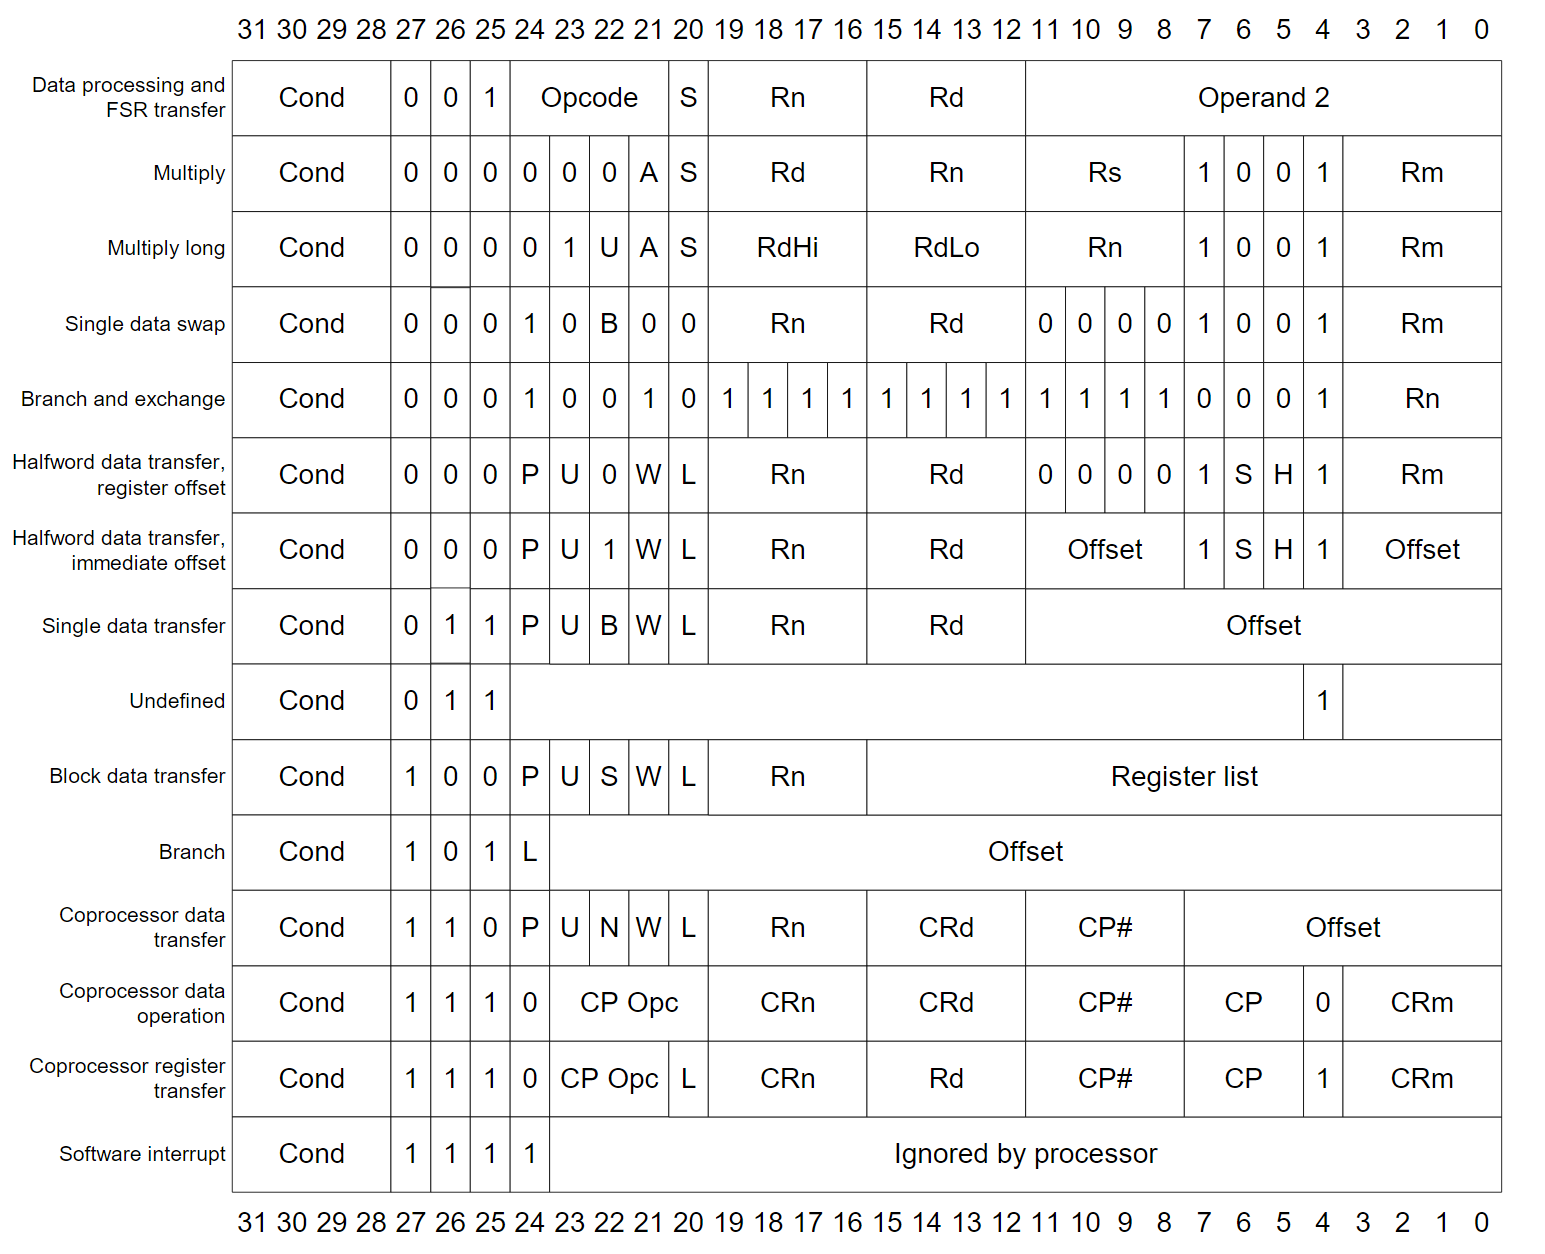
\includegraphics[width=0.85\textwidth]{figure/arm_ist.png}
    \caption{ARM instruction format\cite{arm_ist}.}
    \label{fig:arm_ist}
\end{figure}

However, ARM does not allow users to custom their instructions without the company's permission. Therefore, it has no custom design space for us. What's more, to support more features, ARM has many rarely-used components, which means it is difficult us to implement in only three months.

\item \textbf{RISC-V:} RISC-V is an open standard RISC ISA. Unlike most other ISA designs, the RISC-V ISA is provided under open source licenses that do not require fees to use. Besides, RISC-V is also a newly-emerged ISA. It is first introduced in 2010 and still has a lot of design space to improve. Therefore, it becomes our ideal ISA to choose.

\begin{figure}[!htp]
    \centering
    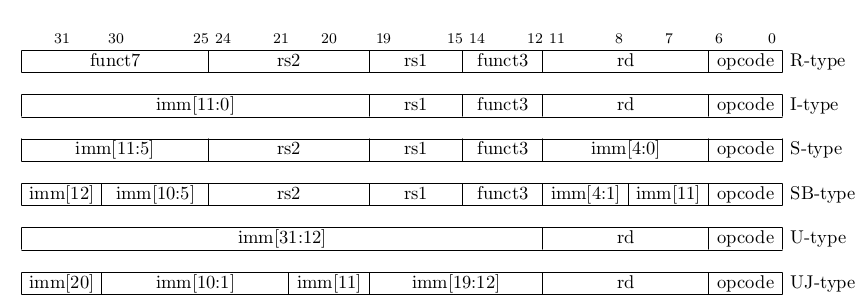
\includegraphics[width=0.85\textwidth]{figure/riscv-isa.png}
    \caption{RISC-V instruction format\cite{RISC-V_unprivileged_ISA}.}
    \label{fig:RISCV_inst}
\end{figure}

However, compared to ARMv7, RISC-V supports less instructions, which means its feature is limited. But, it also means that RISC-V is easier to be implemented.

\end{enumerate}

\section{Microarchitecture} %sl
As mentioned in the previous section, microarchitecture determines the performance, power consumption and also cost of a processor and as a result is key to the success of a processor product. In this section, we use decision matrix to select our microarchitecture design based on customer requirements and engineering specifications. Fig.~\ref{fig:dm-uarch} shows the decision matrix of microarchitecture design.

\begin{figure}[!htp]
    \centering
    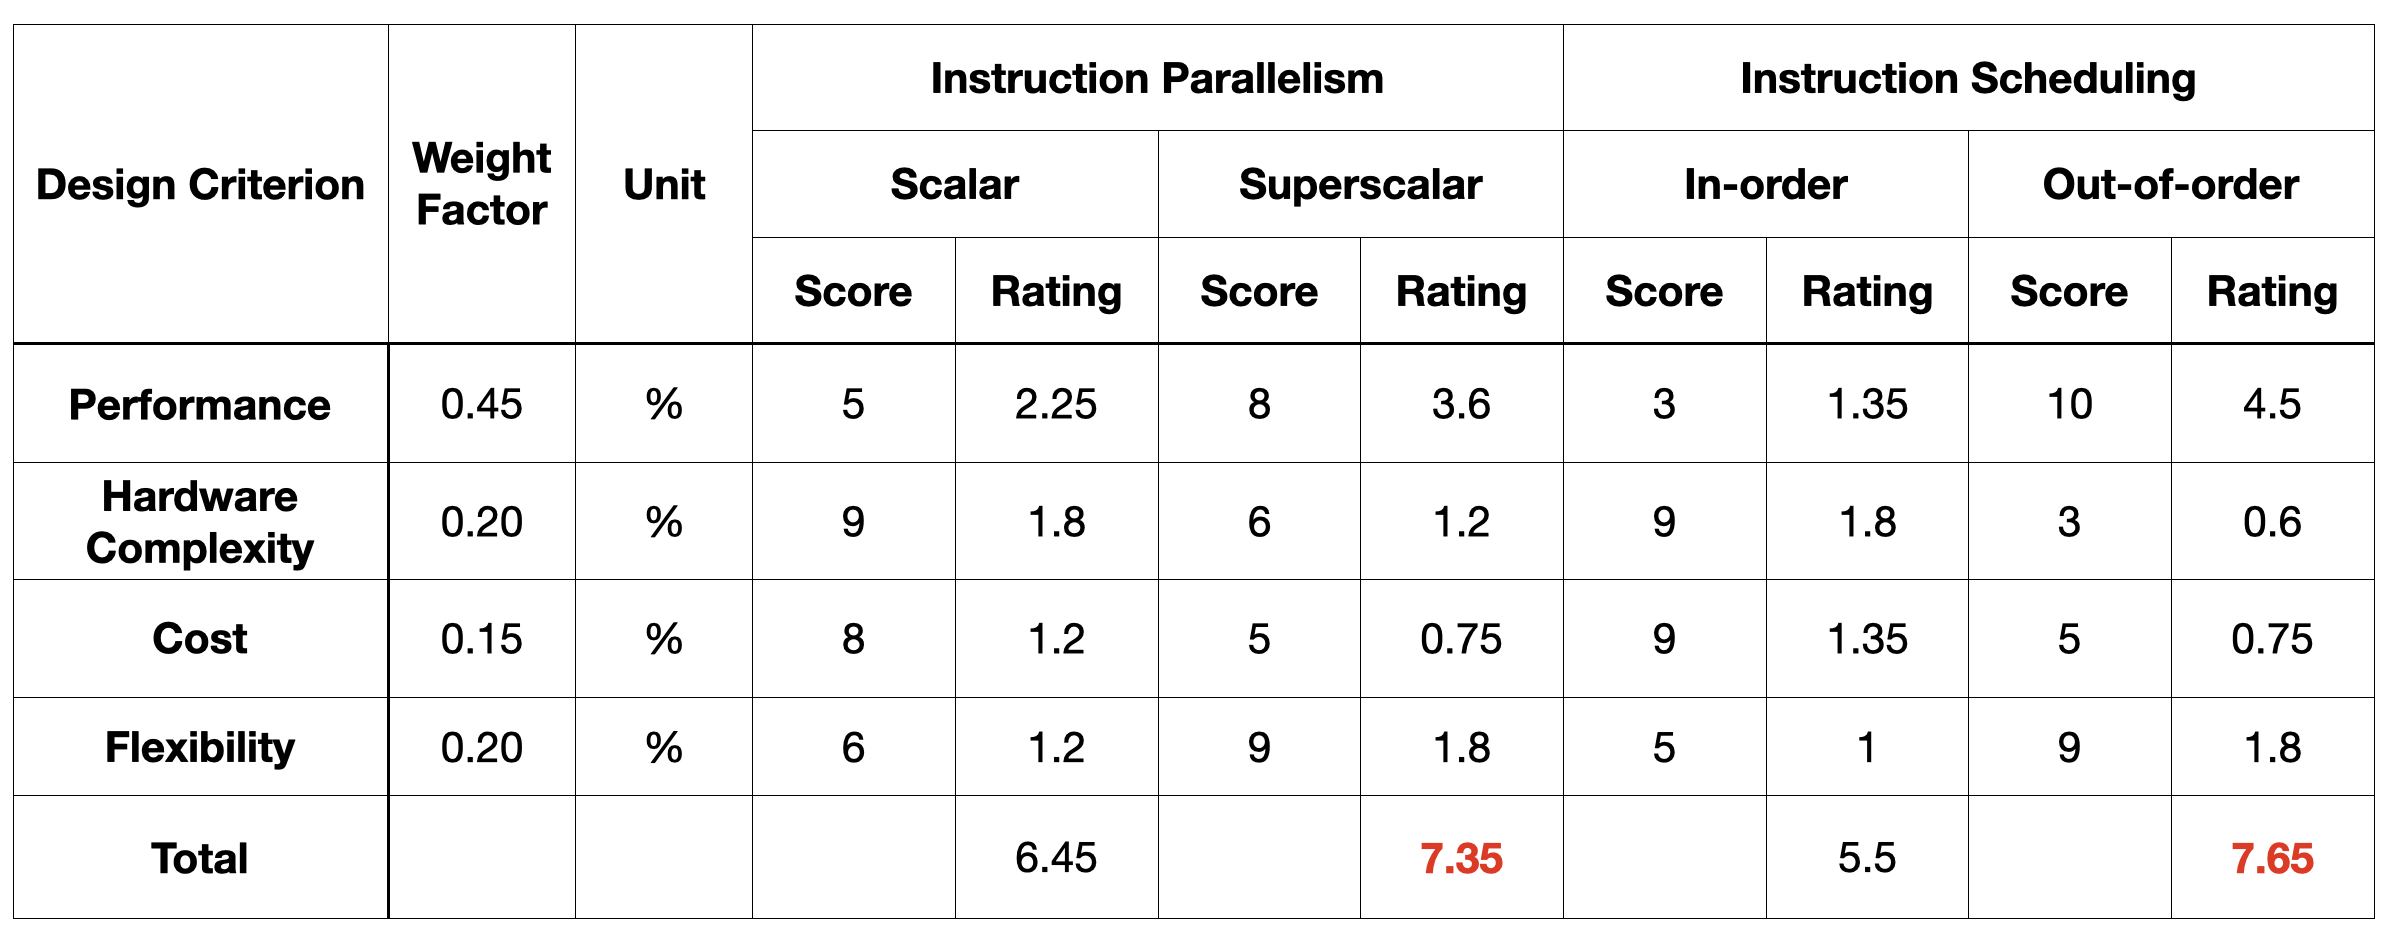
\includegraphics[width=\textwidth]{figure/dm-uarch.png}
    \caption{Decision matrix of microarchitecture design.}
    \label{fig:dm-uarch}
\end{figure}

In the decision matrix, we systematically evaluate our selection on two concepts, i.e., instruction parallelism and instruction scheduling, based on multiple design criterion, including performance, hardware complexity, cost, and flexibility. Based on customer requirements and engineering specifications, we give each criterion a weight factor. As our processor is mainly used for accelerate computing-intensive tasks, performance is the most important evaluation standard, followed by hardware complexity, flexibility and cost. Then, we assess each concept based on a 10-point scale, multiplying by the weight factor and get the rating for each criterion. Finally, we sum the ratings and get the total score of a certain concept design.

For example, in terms of instruction scheduling, in-order design results in good hardware complexity and low cost, but the stalls at different kinds of instruction dependency severely restrict the performance or an in-order processor. On the contrary, the out-of-order design may be complicated to implement in hardware, but results in great performance improvement.

Finally, according to the decision matrix, we choose to implement superscalar and out-of-order features in our processor design.


\section{Verification \& SoC Integration} %yyc

\subsection{Verification}
\subsubsection{Logic Simulation}
We need logic simulator that is free to use, so we have following options:
\begin{enumerate}
    \item \textbf{Vivado Webpack Xsim}. Vivado Webpack Xsim is the simulator used in Vivado IDE. It supports most SystemVerilog features for verification and design. It will provide user good experience if it is used with the Vivado IDE. However, this means it is less flexible.
    \item \textbf{Icarus Verilog}. It is a open-source Verilog / SystemVerilog simulation and synthesize tool. It turns the Verilog / SystemVerilog to some intermediate form to perform synthesize and simulation. It support both the SystemVerilog verification language and design language, but it has low performance for simulation.
    \item \textbf{Verilator}. It is another open-source Verilog / SystemVerilog simulator. It turns Verilog / SystemVerilog models into C/C++ models, and use C++ as the verification language. Although it do not support the verification language of SystemVerilog, it have very good performance for simulation.
\end{enumerate}
There are other commercial software for this task, however, all of them need license which is expensive. Therefore, we make our decision only within the free-to-use ones.

Our final decision is to use both Vivado Webpack Xsim and  Verilator. We use the Vivado Webpack because it is convenient to debug considerably small design in the Vivado IDE. We choose Verilator to simulate the integrated SoC and use Verilator to build our simulation environment. C++ is a much more powerful language than SystemVerilog, and it brings productivity when we build the simulation system. We do not choose Icarus Verilog due to both its poor performance and because it is hard to integrate it with the other parts in the simulation system.

\subsubsection{Functional Verification}
The key part for the functional verification is to choose a proper simulator/ emulator as a comparison model. Followings are some popular choices:
\begin{enumerate}
    \item \textbf{Gem5}. Gem5 is an open source computer architecture simulator used in academia and in industry. It is a very complete and complicate simulator. It provides supports for multiple architecture, including ARM, MIPS, X86, etc. It also provide multiple models for memory system simulation.
    \item \textbf{Qemu}. Qemu is a popular emulator, which dynamically translate the target binary to the host's machine code. Therefore, the user can run RISC-V programs on a X86 machine. This emulator can perform not only user level simulation, but also system level simulation.
    \item \textbf{Spike}. The spike simulator is a lightweight simulator, which implements the RISC-V specification. It is often considered as a golden model for RISC-V specification.
\end{enumerate}

In this project, we focus on the RISC-V ISA. Also, we use the simulator only to verify the functionality correctness of our design, so we do not need a complicated simulator like gem5. Qemu is a emulator so it cannot provide information about program execution trace, which is a critical part to compare to verify our design. Therefore, our final decision is to use spike simulation. Spike is also easier to change to integrate into our simulation system.


\subsection{SoC Integration}
There exists a vast design space for SoC Integration and it is mainly depends on the need. We want our SoC Integration and simulation system makes following tasks more convenient:
\begin{enumerate}
    \item The process of loading and executing program.
    \item The process of reading inputs.
    \item The process of printing message.
    \item The process of saving outputs.
\end{enumerate}
Plus, we want the Integration need less effort. The SoC Integration scheme and the whole simulation system integration scheme is thus referred to Spike. Although spike is an architectural level simulator, its internal structure includes an SoC as well as a well designed, lighted weighted simulation environment.

Figure \ref{fig:450-soc-sys} is a high-level overview of the simulation environment configuration. This figure can serve as a description of the system for both our Verilator-based simulation system as well as the Spike's model, although the internal details are totally different. All the SoC integrate the CPU core with the peripheral devices like RAM and ROM through a system level bus. The simulation environment lies on a host machine, which communicate with the SoC through a pure-software frontend server. The frontend server can perform tasks like load program into the memory as well as proxy some requests from the CPU core. The program running on the CPU can communicate with the front-end server at system level through valuables in the program. The front-end server will link to that register when it loads the program into the RAM. By writing values to and reading values from the valuables, the program can perform tasks like opening a file, writing to a file, etc.

\begin{figure}[!htp]
    \centering
    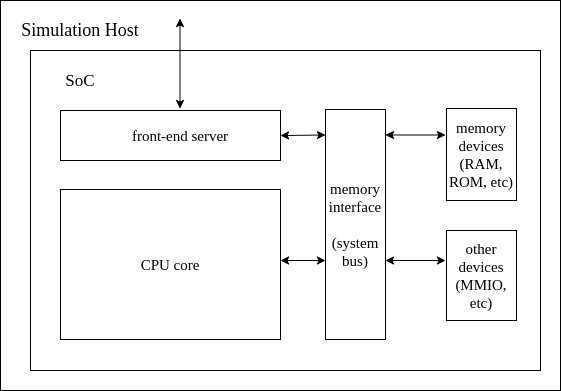
\includegraphics[width=0.8\textwidth]{figure/450-dr3-sys.png}
    \caption{SoC and simulation system integration.}
    \label{fig:450-soc-sys}
\end{figure}
